\documentclass[a4paper,12pt]{article}
\usepackage[utf8]{inputenc}
\usepackage{amssymb,amsmath,uniinput,graphicx,hyperref, multirow,siunitx}
\usepackage[section]{placeins}
\usepackage[ngerman]{babel}
\usepackage{feynmp}
\usepackage[left=3cm,right=3cm,top=3cm,bottom=3cm]{geometry}
\renewcommand{\familydefault}{\sfdefault}
\setlength{\belowcaptionskip}{6pt}
\hypersetup{pdfinfo = {
	Title={Versuchsprotokoll zu Produktion und Zerfall von W-Bosonen},
	Author={Knut Kiesel, Tobias Pook},
	Keywords={W-Bosonen}
}}

% for fenyman graphs
\setlength{\unitlength}{\textwidth}
\def\graphheight{0.15}
\def\graphwidth{.4}

% feynmf with pdflatex compability
\DeclareGraphicsRule{*}{mps}{*}{}

% missing transverse energy
\newcommand{\met}{\ensuremath{\not\mathrel{E}}_T}

% where to find graphics
\graphicspath{{../analyse/}}

\title{Laborpraktikum Teilchenphysik\\ DØ-Experiment: Produktion und Zerfall von W-Bosonen}
\author{Knut Kiesel\\Tobias Pook}
\date{\today}

\begin{document}
\maketitle
\vspace{5cm}
\tableofcontents
\thispagestyle{empty}
\newpage
\setcounter{page}{1}

\section{Ziel des Versuches}
\label{ziel}
Bei diesem Versuch werden aus Daten des DØ Detektors die Masse und die Zerfallsbreite des W-Bosons
sowie den Wirkungsquerschnitt zur Erzeugung und anschließendem Zerfall in zwei Leptonen bestimmt.

Um den Fund des W Bosons am UA2 Experiment zu bestätigen sowie es genauer zu Untersuchen können auch
beim DØ Experiment verschiedene Zerfallskanäle betrachtet werden. Einer von ihnen ist der Zerfall
in ein Elektron/Positron und ein Neutrino. Bei einer Erzeugung des W Bosons mit Valenzquarks der
Protonen/Antiprotonen ergibt sich der Feynmangraph in erster Ordnung in Abbildung
\ref{fig:feynman}.
\begin{figure}[h]
\centering
\begin{fmffile}{feymanE}
	\begin{fmfgraph*}(\graphwidth,\graphheight)
		\fmfleft{i2,i1}
		\fmfright{o2,o1}
		\fmf{fermion,label=$d$}{i1,v1}
		\fmf{fermion,label=$u$}{v1,i2}
		\fmf{photon,label=$W^-$}{v1,v2}
		\fmf{fermion,label=$ν$}{o1,v2}
		\fmf{fermion,label=$e$}{v2,o2}
	\end{fmfgraph*}
\end{fmffile}
\begin{fmffile}{feymanE+}
	\begin{fmfgraph*}(\graphwidth,\graphheight)
		\fmfleft{i2,i1}
		\fmfright{o2,o1}
		\fmf{fermion,label=$u$}{i1,v1}
		\fmf{fermion,label=$d$}{v1,i2}
		\fmf{photon,label=$W^+$}{v1,v2}
		\fmf{fermion,label=$e$}{o1,v2}
		\fmf{fermion,label=$ν$}{v2,o2}
	\end{fmfgraph*}
\end{fmffile}
\caption{Feynman Diagramm für die Erzeugung von W-Bosonen durch zwei Quarks der ersten Familie und
Vernichtung in zwei Leptonen.}
\label{fig:feynman}
\end{figure}

Den Wirkungsquerschnitt kann man mit
\begin{align}
\label{form:xstot}
	σ = \int_0^1dx_p\int_0^1dx_{\bar{p}} \sum_{i,j} f_i(x_p)f_j(x_{\bar{p}}) \hat{σ}
\end{align}
berechnen, wobei
\begin{align*}
	\hat{σ} = \frac{1}{N_C}\frac{12π}{m_W^2}\frac{Γ_{qq'}Γ_{eν}}{Γ^2_W}
	\frac{ x_px_{\bar{p}} s Γ_W^2}{\left( x_px_{\bar{p}}s - m_W^2\right)^2 + m_W^2Γ_W^2}
\end{align*}
und
\begin{align*}
	Γ_{ff'} = \frac{N_C}{12} \frac{α}{\sin^2θ_W}m_W
\end{align*}
ist. Dabei sind $f_i$ die Patron-Dichte-Funktionen, $N_C$ die Anzahl an Farben und $\sqrt{s}$ die
Schwerpunktsenergie.
Unter der Annahme, das W kann nur in drei Leptonfamilien und zwei Quarkfamilien zerfallen (das
top-Quark ist zu schwer), kann man über obrige Formel die gesamte Zerfallsbreite des W ausrechnen:
\begin{align}
\label{form:width}
	Γ_W = 3Γ_{eν} + 2Γ_{ud}  = \frac{ 3+2N_C}{12} \frac{α}{\sin^2θ_W}m_W
\end{align}
Damit ergibt sich für
\begin{align}
\label{form:xscms}
	\hat{σ} = \frac{πα²}{12\sin^4θ_W} \frac{ x_px_{\bar{p}} s }{\left( x_px_{\bar{p}}s -
	m_W^2\right)^2 + m_W^4\frac{(3+2N_C)^2}{12^2}\frac{α^2}{\sin^4θ_W}}.
\end{align}

Über die Masse des W Bosons kann man den elektroschwachen Mischungswinkel, oder auch Weinbergwinkel
$θ_W$ genannt, berechnen:
\begin{align}
	\label{form:wein}
	\cosθ_W = \frac{m_W}{m_Z}
\end{align}
In dem Versuch werden die Masse des Z Bosons $m_Z$ sowie die Feinstrukturkonstante $α$ als gegeben
vorausgesetzt.

\section{Vergleich von Simulation und Daten}

Im Detektor kann die W Masse nicht direkt gemessen werden, sondern nur manche Tochterteilchen. In
dem hier untersuchtem Prozess sind dies ein leichtes geladenes Lepton $e$
\footnote{Elektron wird ab nun als Synonym für Elektron und Positron benutzt} sowie
ein Neutrino $ν$
\footnote{Neutrino wird als Synonym für (Anti-)elektronneutrino benutzt}. Da die
longitudinale Anfangsbedinungen nicht bekannt sind, werden
nur transversale kinematische Größen betrachtet. Für die Auswertung werden Daten aus dem Kalorimeter
denen des Spurdetektors bevorzugt, da der Kalorimeter die kleinere Unsicherheit hat. So wird zum Beispiel
die transversale Energie eines Elektrons/Positrons
\begin{align*}
	E_{T} = E\sin\left( 2\arctan\left( e^{-\eta} \right) \right)
\end{align*}
aus der Energie im Kalorimeter $E$ und $\eta$ berechnet, wobei $\eta$ sowohl Informationen aus
Spurdetektor und Kalorimeter enthält.
Die Fehlende Transversale Energie wird komplett aus dem Kalorimeter bestimmt und berechnet sich
durch
\begin{align*}
	\met = \sqrt{ \not\mathrel{E}^{2}_{x} + \not\mathrel{E}^{2}_{y}}
\end{align*}
wobei $\not\mathrel{E}$ als
\begin{align*}
	\not\mathrel{E}_i = \left| - \sum E\vec{e_i} \right|
\end{align*}
definiert ist. Da das Neutrino im Detektor nicht nachgewiesen wird sondern ohne Interaktion den
Detektor verlässt, wird $\met$ als Neutrinoenergie
benutzt. Da nur die transversalen Komponenten von Elektron und Neutrino verwendet werden, kann auch
nur die invariante transversale Masse der Leptonen und damit des W Bosons berechnet werden.
\begin{align*}
	m_T = \sqrt{2E_T\met\left( 1-\cos(Δφ_{e,ν}) \right)}\hspace{0.3cm}\footnotemark
\end{align*}
\footnotetext{Da die beobachteten transversalen Elektronenergien größer als einige $\si{GeV}$ sind, wird
im Folgenden die Elektronmasse vernachlässigt.}

\subsection{Beschreibung der simulierten Daten}
Um Untergründe zu entfernen ist es hilfreich die gemessenen Daten mit simulierten Ereignissen zu
vergleichen. Da die W Masse im voraus noch nicht bekannt ist, werden Ereignisse für unterschiedliche
W Massen generiert.
Weil man den Untergrund durch $W\rightarrow τν_τ\rightarrow eν_τν_τν_e$ in Daten schlecht filtern kann,
sind auch $τ$ Ereignisse simuliert.

Die Qualität der Simulation ist aber eher durchwachsen, da gewisse Größen wie zum Beispiel der
Abstand des Vertices zum Ursprung, der Polarwinkel $φ$ oder die Elektronisolation sehr schlecht
beschrieben werden.

\begin{figure}[h]
	\centering
	\newcommand{\halftext}{0.49\textwidth}
	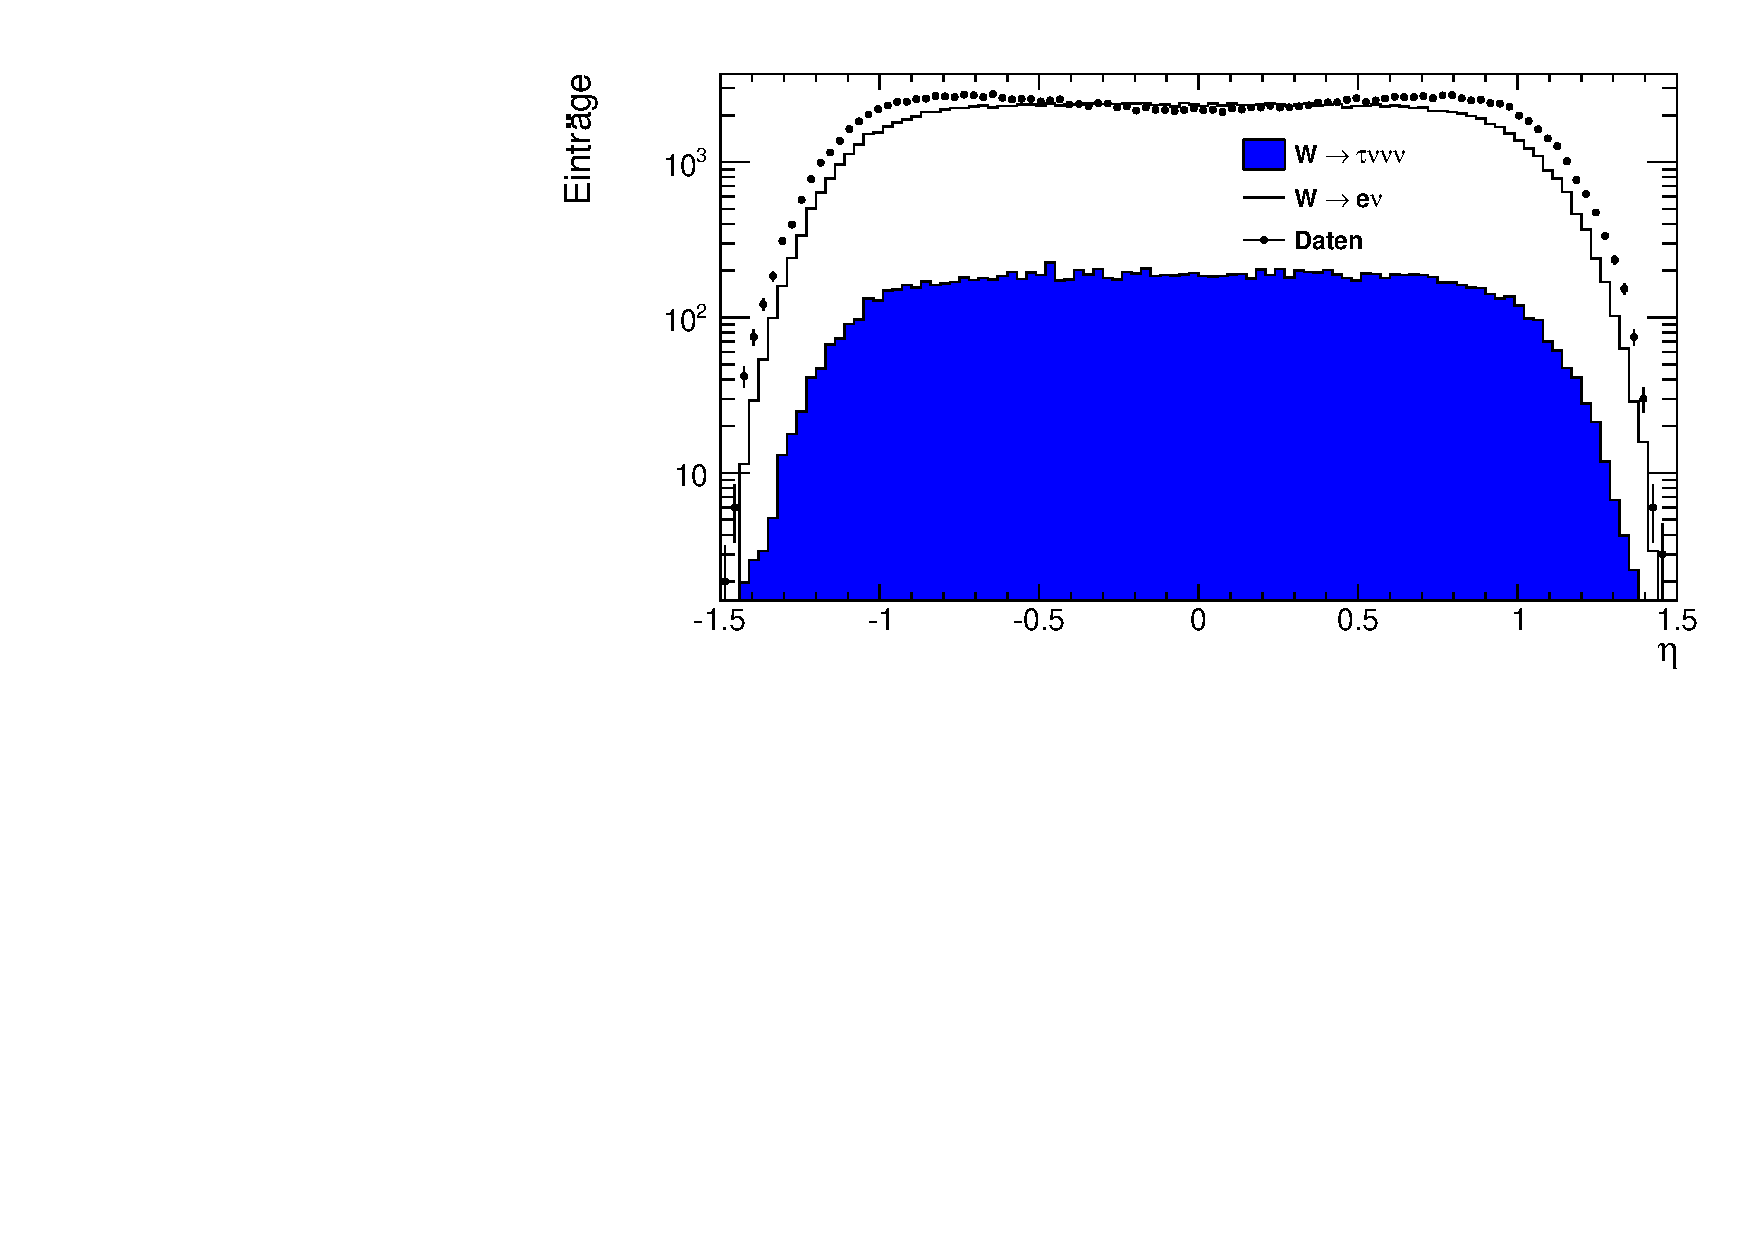
\includegraphics[width=\halftext]{eta.pdf}
	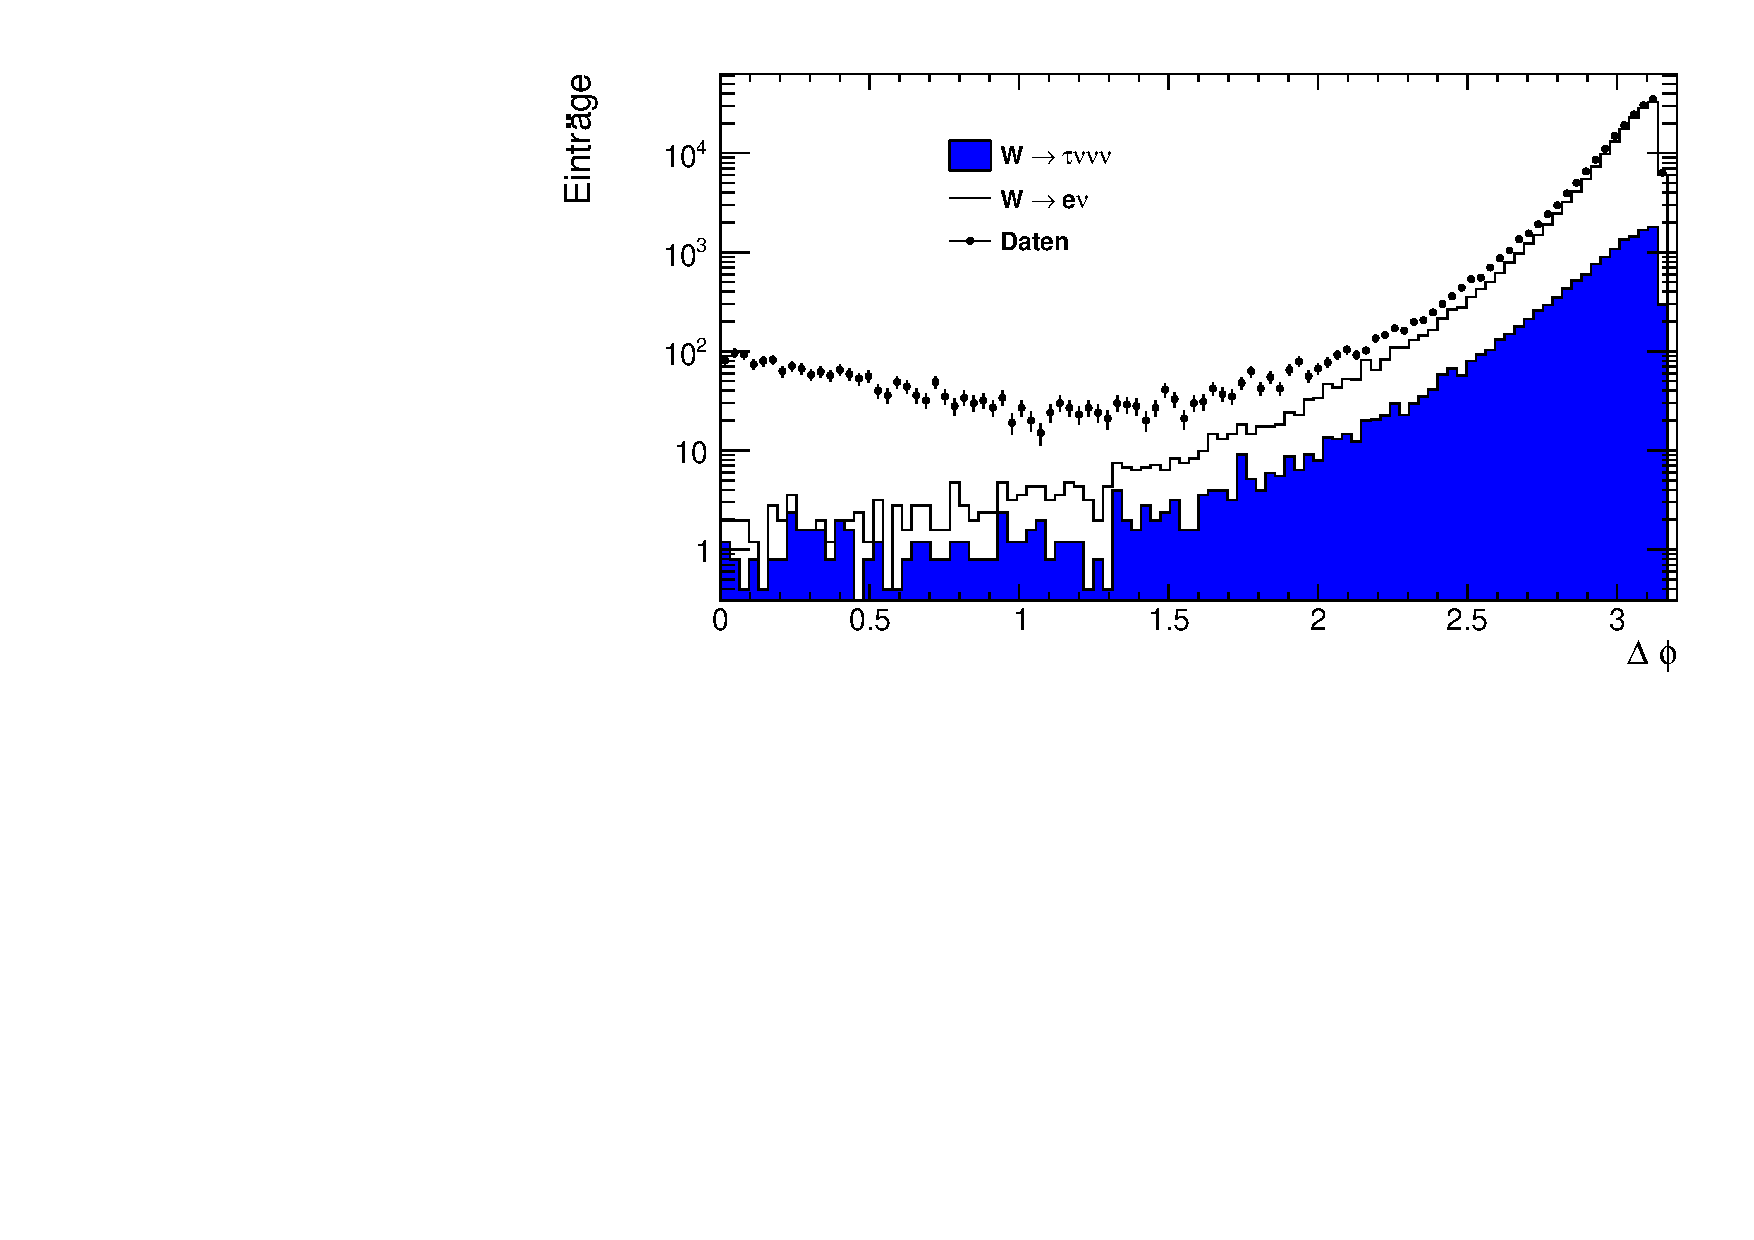
\includegraphics[width=\halftext]{delta_phi.pdf}\\
	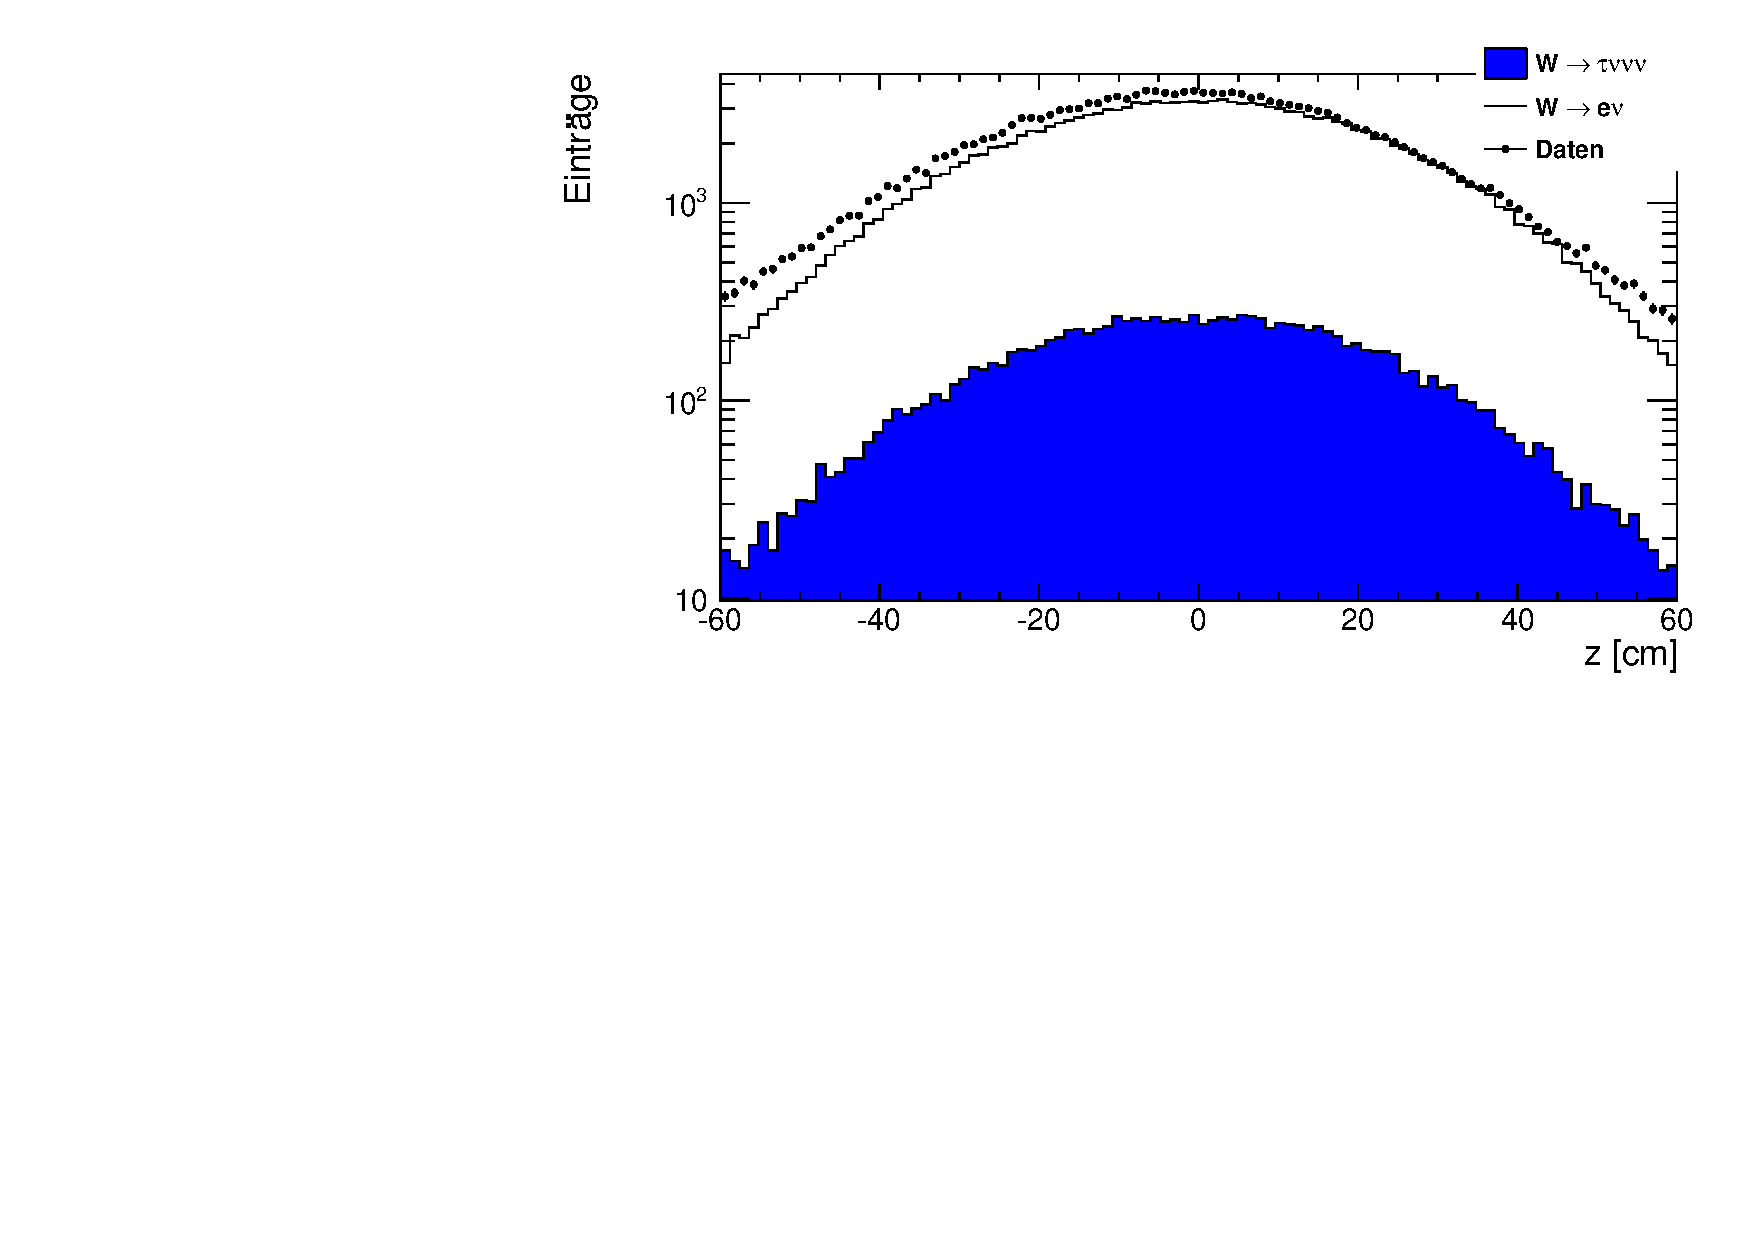
\includegraphics[width=\halftext]{vertex_z.pdf}
	\includegraphics[width=\halftext]{enengy_fraction.pdf}\\
	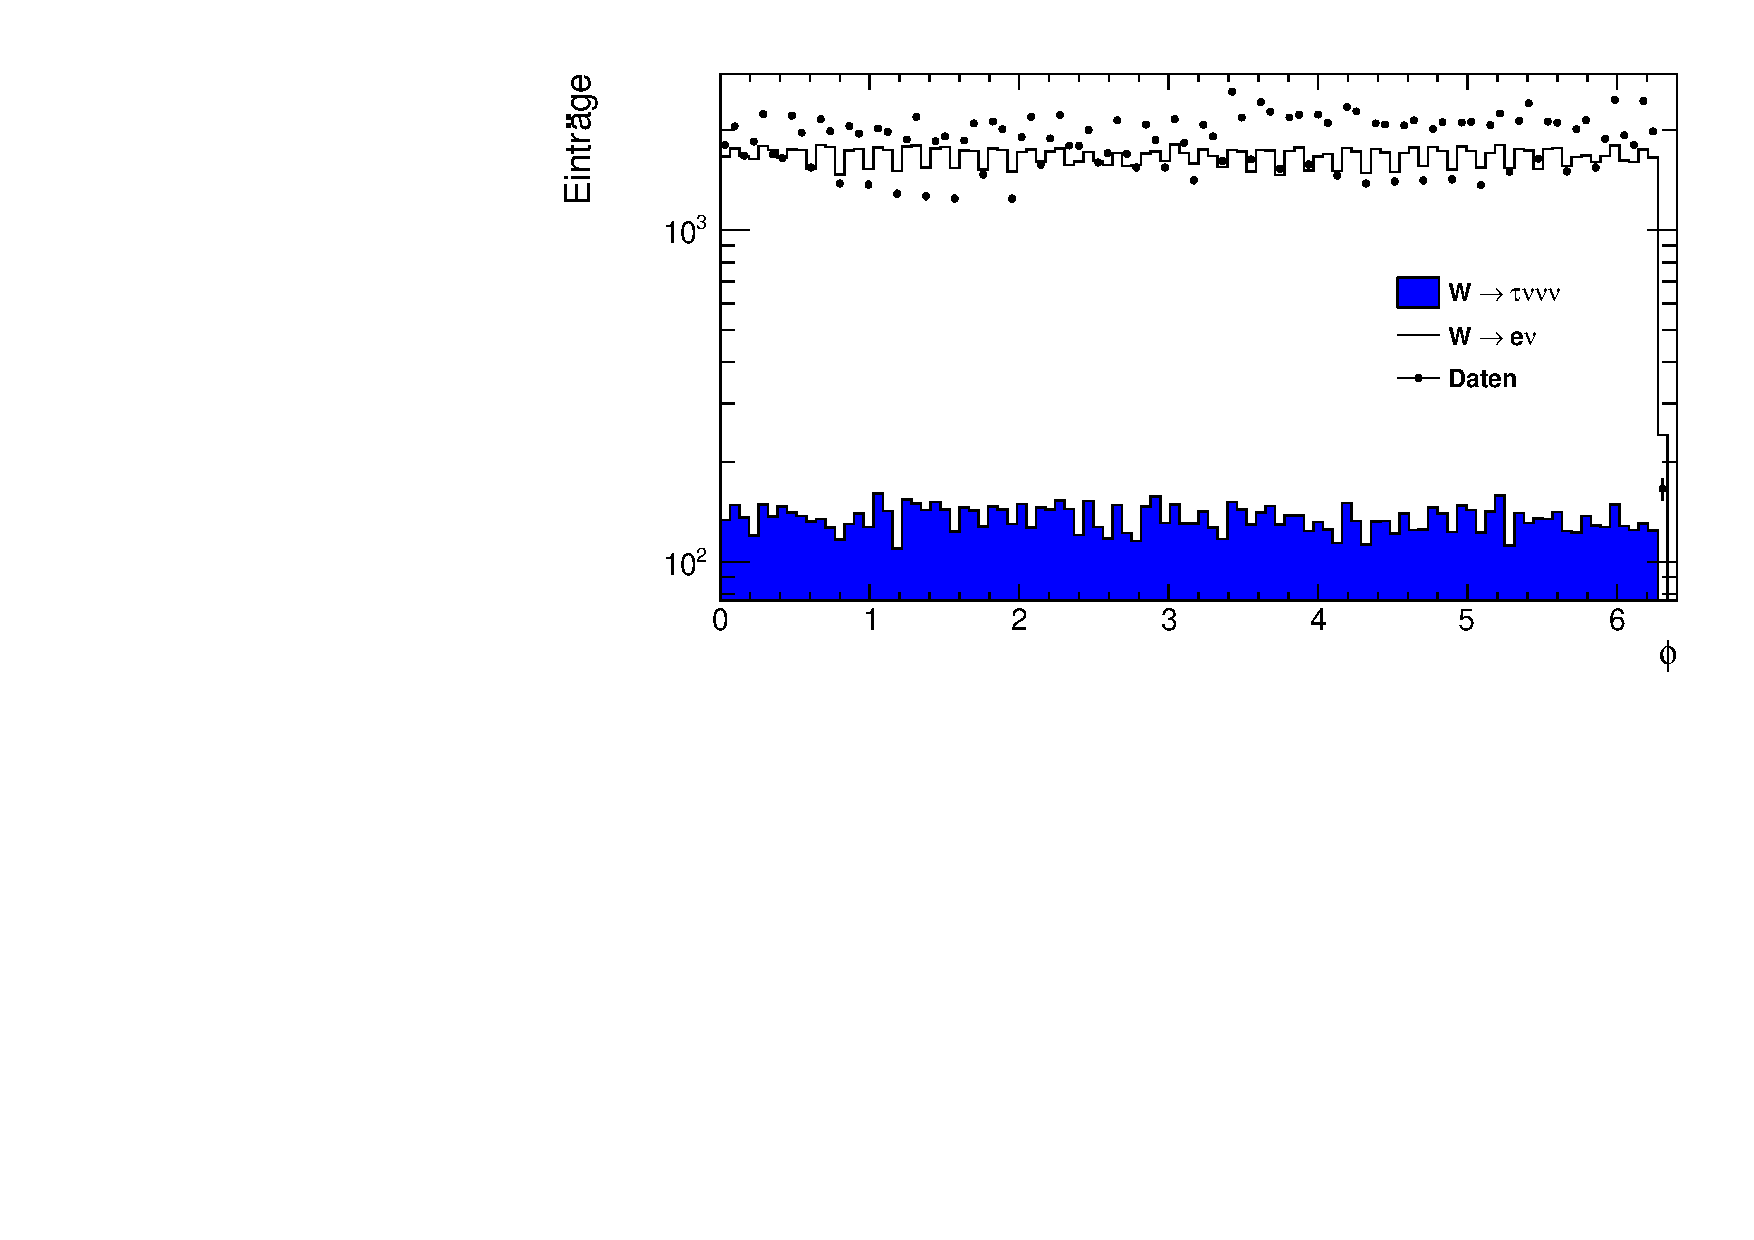
\includegraphics[width=\halftext]{phi.pdf}
	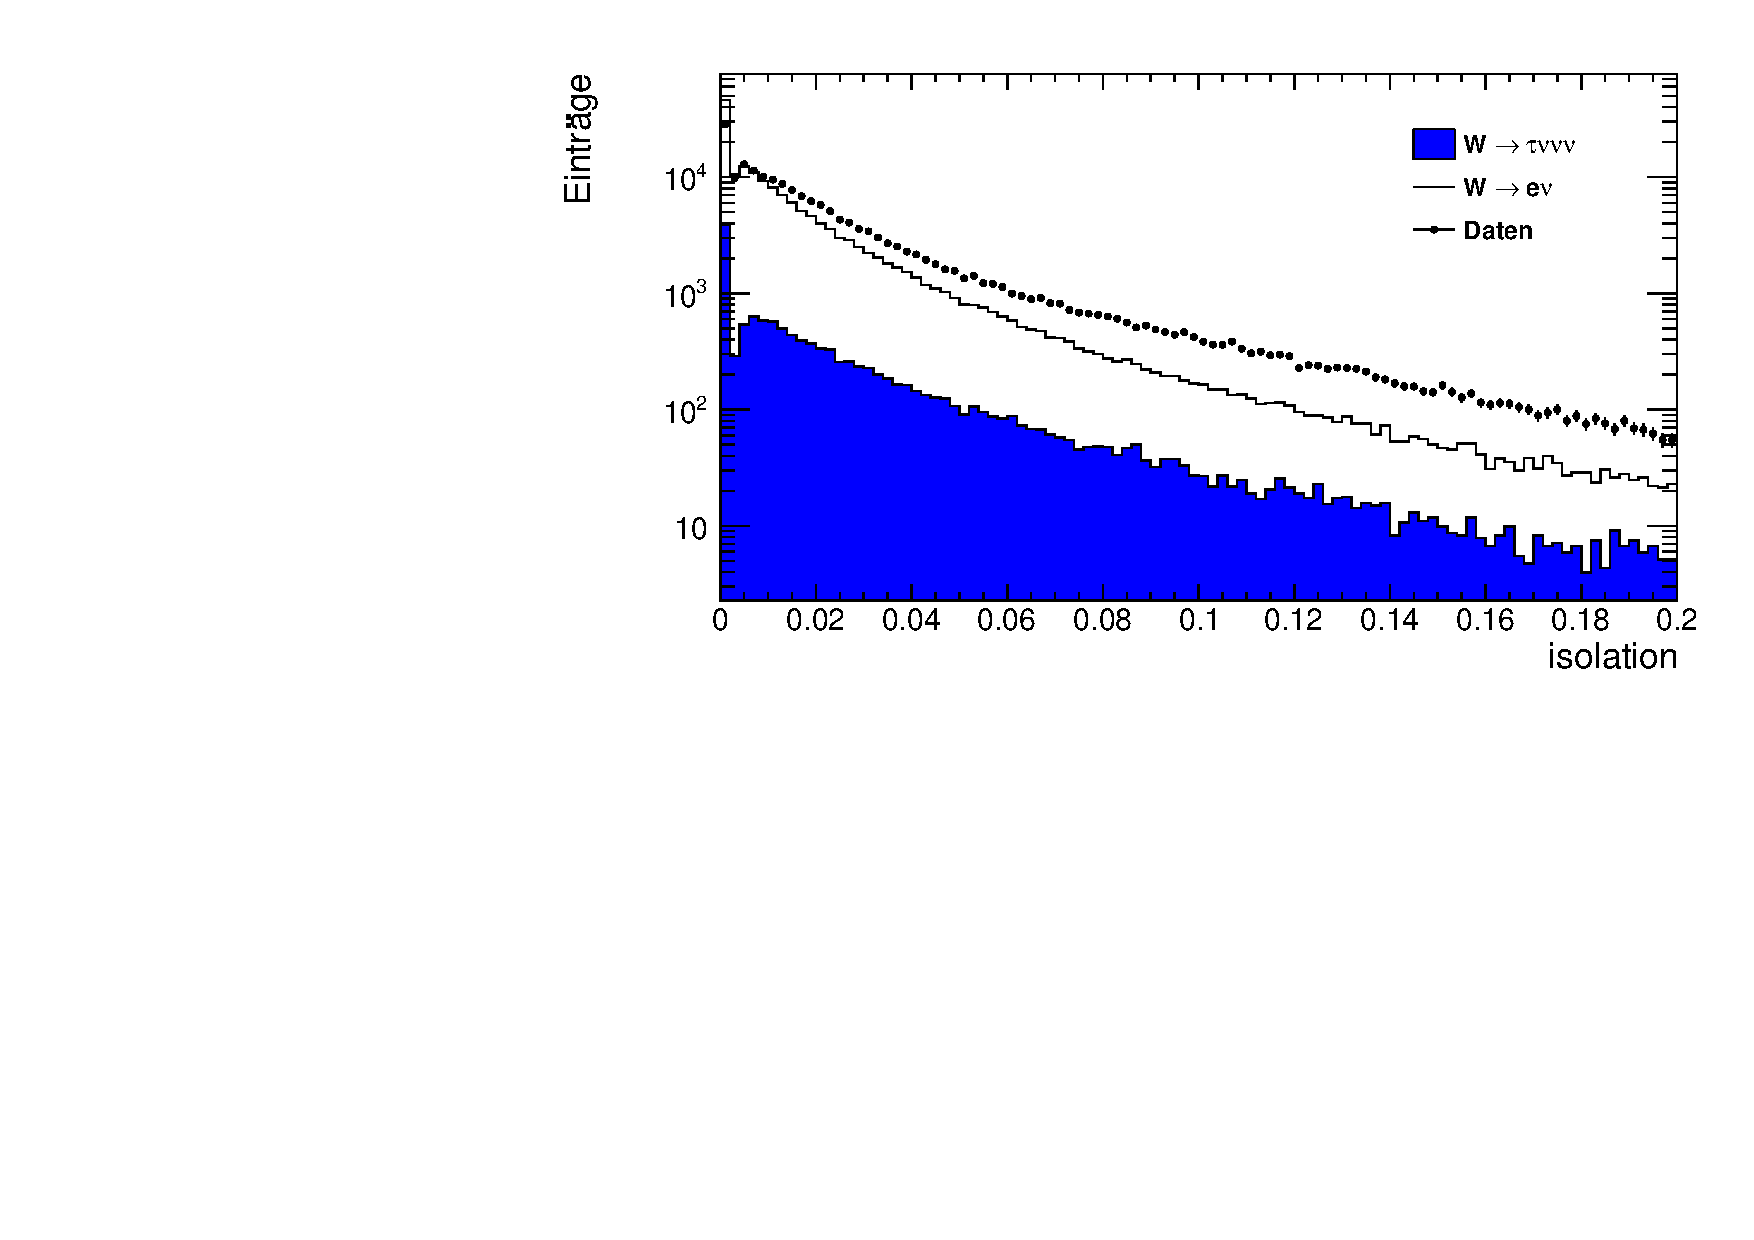
\includegraphics[width=\halftext]{isolation.pdf}\\
	\caption{Die Verteilung der Rapidität $η$, Winkel zwischen den Leptonen $Δ\phi$, der Abstand vom Ursprung in
	Strahlrichtung $z$, der Anteil der Energie im Kalorimeter, der Polarwinkel $\phi$ und die
	Elektronisolation für Daten und Simulation. }
	\label{fig:variables}
\end{figure}

Einige der Größen werden in Abbildung \ref{fig:variables} dargestellt. Man sieht die $τ$ Ereignisse
als blaues Histogram, die übrigen simulierten Daten als schwarzes Histogram und die Daten als
Punkte. 
\subsubsection*{Normierung der simulierten Daten}
Die Simulierten Ereignisse müssen, um einen Vergleich mit den gemessenen Daten zu ermöglichen, auf die
integrierte Luminosität der Daten von $\mathcal{L}_{int}=198 \pm \SI{20}{pb^{-1}}$ normiert werden.
Dazu werden die Monte Carlo Sample, nach den Vorgaben aus \cite{versuchsanleitung},
in Abhängigkeit der Anzahl ursprünglich generierter Monte Carlo (\textbf{MC}) Ereignisse $N_{gen}$, mit einem Faktor:
\begin{align*}
	\textsl{w}= \frac{\sigma \mathcal{L}_{int}}{N_{gen}} \cdot 0.9
\end{align*}
skaliert. Der Faktor $0.9$ beschreibt einen Korrekturterm, der eine, im Vergleich zum realen Detektor,
zu hoch angenommene Auflösung und Nachweiseffizienz bei der Generierung der MC Ereignisse berücksichtigt.


\subsection{Selektion der Daten}
Da nicht alle aufgezeichneten Ereignisse dem zu untersuchendem Prozess zugrunde liegen, müssen die
Daten gefiltert werden, möglichst ohne viele richtige Ereignisse zu verlieren. Es werden nur
Elektronen betrachtet, deren Schauer wie eine elektromagnetische und nicht wie eine hadronische
Kaskade aussieht. Zu dem Schauer muss sich auch in kleinem Abstand eine Spur im Spurdetektor befinden.
Die Elektronen müssen isoliert sein, in $|\eta| < 1.1$ liegen. Es dürfen in dem Ereignis keine
hadronischen Jets mit einem Transversalimpuls von über $\SI{15}{GeV}$ vorkommen und der Primärvertex
darf entlang der Strahlachse nur $\SI{60}{cm}$ vom Mittelpunkt abweichen. Diese Auswahl wird immer
getroffen und nicht gesondert erwähnt wenn angewandt.

Hierzu werden die simulierten und gemessenen Daten in normierte Histogrammen übereinandergelegt
und die Unterschiede durch geeignete Schnitte versucht zu verringert. Ziel ist vor allem eine gute
Übereinstimmung in $m_T$, da daraus die Masse bestimmt wird. Die Abschätzung von Selektionsgrenzen
wird in Abbildung \ref{fig:abschaetzung} veranschaulicht. Links oben sieht man die transversale
invariante Masse ohne Einschränkungen. Die Verteilungen von Daten und Simulation unterscheiden sich
noch deutlich. Rechts oben sieht man die Verteilung der transversalen
fehlenden Energie. Da Daten und Simulation rechts der gezeichneten Linie gut übereinander stimmen,
wird in Zukunft gefordert, dass $\met > \SI{30}{GeV}$ sein muss. Im Bild links unten sieht man die
Verteilung der transversalen Elektronenergie und die Grenze, ab der Daten und Simulation hier
übereinstimmen. Zuletzt wird rechts unten wieder $m_T$ gezeigt.

\begin{figure}[h]
	\centering
	\includegraphics[width=.49\textwidth]{mwt1tau.pdf}
	\includegraphics[width=.49\textwidth]{met1tau.pdf}\\
	\includegraphics[width=.49\textwidth]{el_etmet>30tau.pdf}
	\includegraphics[width=.49\textwidth]{mwtmet>30&&el_et>30tau.pdf}
	\caption{Abschätzung der Selektionsgrenzen mit Vergleich von Daten und Simulation. In Blau ist
	der $τ$ Untergrund eingezeichnet. Die Simulation wird hier mit der generierten W Masse von
	$\SI{80.3946}{GeV}$ erzeugt.}
	\label{fig:abschaetzung}
\end{figure}

In Blau sieht man in jedem Bild Ereignisse, in denen das W ein $τ$ und ein $ν_τ$ erzeugt. Das $τ$
zerfällt nach sehr kurzer Zeit wieder in ein $e + ν_e + ν_τ$. Da man die Neutrinos nicht einzeln
Messen kann sondern nur die fehlende Energie, die durch alle Neutrinos zusammen verursacht wird,
kann man diese Ereignisse kaum Filtern, sondern muss den Untergrund über Simulationsvergleiche
abschätzen. Während am Anfang der Anteil der $τ$ Ereignisse noch 8.8\% beträgt, sind es nach beiden
Schnitten 1.1\%.

Da die wahre W-Masse unbekannt ist, kann man die Schnitte noch auf andere simulierte Datensätze
optimieren. Es folgt ein Fehler auf die Schnitte von $\SI{5}{GeV}$.

Der Versuch auf die Elektronenisolation, den Abstand des Primärvertex oder ähnliche Variablen zu
schneiden wird aufgegeben, da es dort sehr schwer ist die Simulation und die Daten übereinander zu
bringen. Dies liegt unter anderem an der oben Beschriebenen schlechten Generation der Simulation.
Die gewählten Schnitte sorgen für ein gutes Übereinander stimmen von Daten und Simulation, ohne dass
die Effizient zu niedrig wird.

\newpage
\section{Bestimmung der Masse des W Bosons}
\subsection{Template Methode zur Bestimmung der W Masse}
Zuerst muss die Übereinstimmung von Simulation und Daten quantifiziert werden.

Da das skalieren der Simulierten Daten einen großen Fehler mit sich bringt und auch nach dem
skalieren die gesamten Ereigniszahlen stark voneinander abweichen, ist es nötig, die Histogramme zu
normieren. Dies wiederum hat zur Folge, dass man den $χ²$ Test für gewichtete Histogramme benutzen
muss\cite{cramer1999mathematical}.
Weiterhin müssen in einem Bin genug
Einträge sein (mehr als 9), damit man die poissonverteilten Einträge in eine Gaußverteilung 
übergehen und man den Fehler als Quadratwurzel der Einträge benutzen kann. Außerdem verringert man
somit die relative Gewichtung von Bins mit zu wenig Einträgen.



Eine Schwierigkeit besteht weiterhin in dem Wählen der Anzahl der Bins sowie den verwendeten
Bereich. Im Allgemeinen steigt das $χ²$ mit zunehmender Anzahl Bins. Die Anzahl der Bins wird auf
20 gesetzt, da dort der statistische Fehler klein ist, die Struktur der Verteilung aber nicht
verloren geht. Der Bereich wird möglichst groß gewählt, ohne dabei Bins mit weniger als 10 Einträge
mitzunehmen.

Trägt man nun für jede simulierte Masse das $χ²/\text{NDF}$ aus dem Vergleich zwischen der
Verteilung von $m_T$ von
Simulation und den Daten auf, erhält man wie in Abbildung \ref{fig:template} zu sehen eine Parabel.

\begin{figure}[htb]
	\centering
	\includegraphics[width=1\textwidth]{template.pdf}
	\caption{Template Methode mit den Bedingung $\met > \SI{30}{GeV}$ und $E_{T} > \SI{30}{GeV}$. Die gesuchte W Masse befindet sich im Minimum der Parabel, da dort
		das $χ²/\text{NDF}$ minimal ist.}
	\label{fig:template}
\end{figure}
% minimum bei 1

Für die am Besten passende W Masse muss das $χ²/\text{NDF}$ möglichst klein sein. Man passt an den
Graphen in Abbildung \ref{fig:template} deshalb eine Parabel an und bestimmt deren Minimum. Die
Fehler sowie das $χ^2/\text{NDF}$ der Anpassung sind nicht von Bedeutung, da die Punkte keine
Fehler besitzen nur ein ROOT interner Standardfehler gesetzt wird.

Da das Minimum der Parabel nahe $1$ liegt, ergibt sich der statistische Fehler der W Masse aus der Abweichung vom Minimum beim Erhöhen des
$χ²/\text{NDF}$ um $1$.

Wenn man eine Parabel der Form $a + bx + cx²$ anpasst, erhält man somit $m_w = -\frac{b}{2c} ±
\frac{1}{\sqrt{c}}$.
Damit ergibt sich mit den Schnitten $\met > \SI{30}{GeV}$ und $E_{T} > \SI{30}{GeV}$
\begin{align*}
	m_W =  ( 80.36 ± 0.25  ) \si{GeV}.
\end{align*}

Beim Variieren der Selektionsgrenzen, des Vergleichbereichs und der Anzahl Bins ändert sich der
eigentliche Wert der W Masse kaum, wohl aber der statistische Fehler. Er wird deshalb mit einer
Unsicherheit von $^{+0.8}_{-0.05}\si{GeV}$ abgeschätzt.

\subsection{Systematische Fehler bei der W-Massenbestimmung}
\label{sysunc}
Im folgenden werden die berücksichtigten systematischen Fehler bei der W Massenbestimmung quantifiziert und zu einem systematischen Gesamtfehler 
addiert.
\subsubsection*{Energieskala von $E_{T}$}
Die Bestimmung der Skala der Transversalenergie des Elektrons besitzt nach \cite{Abachi:1996ey} eine relative Unsicherheit von ca. $2\%$. Um den systematischen Einfluss
dieser Größe auf das Endergebnis zu bestimmen wurden alle $E_{T}$ Werte entsprechend dieser relativen Unsicherheit nach oben und unten variiert und die
W Masse Erneut bestimmt. Die Abweichungen sind in Tabelle \ref{tab:syset} zusammengefasst. Damit lässt sich der mittlere systematische Fehler durch die 
Wahl der transversalen Energieskala zu $0.3MeV$ bestimmt.
\begin{table}[h]
	\centering
	\begin{tabular}{c| c c c}
		$\frac{\Delta E_{T}}{E_{T}}$ & $M_{W} [GeV]$ & $\Delta M_{W}$ &$\frac{\Delta M_{W}}{M_{W}}$\\
		\hline
		$2\%$ & $81.56\pm 0.26$ & 1.03 & $1.2\%$\\
		$0\%$ & $80.53\pm 0.3$ & 80.60 & $0\%$ \\
		$-2\%$ & $79.56\pm 0.3$ & 80.19 &$1.2\%$ 
	\end{tabular}
	\caption{Verschiebung der transveralen Elektronenenergieskala um $2\%$}
	\label{tab:syset}
\end{table}
\subsubsection*{Energieskala von $\met$}
Analog zum vorherigen Abschnitt wird nun auch die fehlende transversale $\met$ um $2\%$  variiert. Die Wahl dieser Abweichung wird dadurch begründet, dass
die Selektion hoch energetische Jets ausschließt und in der Berechnung $\met = - \sum \vec{E}_{T}$ die Unsicherheit einen dominanten Anteil spielt.
Die Ergebnisse der Variation sind in Tabelle \ref{tab:sysmet} zusammengefasst. Damit lässt sich der mittlere systematische Fehler durch die 
Wahl der Energieskala der fehlenden transversalen Energieskala zu $0.3MeV$ bestimmt.
\begin{table}[h]
	\centering
	\begin{tabular}{c| c c c}
		$\frac{\Delta E_{T}}{E_{T}}$ & $M_{W} [GeV]$ & $\Delta M_{W}$ &$\frac{\Delta M_{W}}{M_{W}}$\\
		\hline
		$2\%$ & $81.56\pm 0.26$ & 1.03 & $1.2\%$\\
		$0\%$ & $80.53\pm 0.3$ & 80.60 & $0\%$ \\
		$-2\%$ & $79.56\pm 0.3$ & 80.19 &$1.2\%$ 
	\end{tabular}
	\caption{Verschiebung der fehlenden transveralen Elektronenenergieskala um $2\%$}
	\label{tab:sysmet}
\end{table}
\subsubsection*{Variation der Selektionsgrenzen}
Um den Einfluss der gewählten Selektionsgrenzen zu bestimmen, werden diese um $\SI{5}{GeV}$
variiert. Es ergeben sich die Verschiebungen in Tabelle \ref{tab:variation}, mit denen der systematisch Fehler
auf die W Masse zu $\SI{0.5}{GeV}$ abgeschätzt wird, indem die halben Abweichungen quadratisch addiert werden.
\begin{table}[h]
	\centering
	\begin{tabular}{c| c c c}
		$E_{T} \backslash \met$ & 15 & 20 & 25 \\
		\hline
		15 &  & 80.89 & \\
		20 & 79.94 & 80.60 & 80.53 \\
		25 &  & 80.19 &
	\end{tabular}
	\caption{Verschiebung der Selektionsgrenzen um $\SI{5}{GeV}$}
	\label{tab:variation}
\end{table}
\subsubsection*{Kombination der systematischen Fehlerquellen}
Das Berechnen des systematischen Gesamtfehler geschieht in 2 Schritten:
die Unsicherheiten auf $E_{T}$ und $\met$ sind, wie in Abbildung \ref{fig:etVSmet} zu erkennen ist, stark korreliert (Korrelationskoeffizient $0.85$)
und werden deshalb zunächst linear addiert. Die Unsicherheit durch die Wahl der Selektionsgrenzen wird (auch wenn das sicherlich nicht ganz korrekt ist)
als unabhängig angesehen und zu dem gemeinsamen Fehler der Energieskalenbestimmung quadratisch addiert. Damit ergibt sich als abschließendes Ergebnis der 
W Massenbestimmung:
\begin{align*}
	m_W = ( 80.32 ± 0.27 (stat.) ± 0.78(sys.)) \si{GeV}
\end{align*}
\begin{figure}[htb]
	\centering
	\includegraphics[width=1\textwidth]{correlation_metVSel_et.pdf}
	\caption{Grafische Darstellung der Korrelation zwischen $E_{T}$ und $\met$ mit in rot eingezeichneten Selektionsgrenzen}
	\label{fig:etVSmet}
\end{figure}

\subsection{Überprüfung der Ergebnisse durch Untersuchung einer Kontrollvariablen}
Um die Unsicherheiten der Analyse von $m_{T}$ besser abschätzen zu können und das Ergebnis zu überprüfen wird zusätzlich
die Übereinstimmung der $E_T$ Verteilungen verglichen und daraus mit der Template Methode die W Masse
berechnet. Eine einfache Mittelung der Werte ist nicht möglich, da $m_T$ und $E_T$ stark korreliert
sind, wie man in Abbildung \ref{fig:correlation} sehen kann.
\begin{figure}[htb]
	\centering
	\includegraphics[width=.49\textwidth]{correlation_mwtVSel_et.pdf}
	\includegraphics[width=.49\textwidth]{correlation_mwtVSel_etmwt_el_et>1_7.pdf}
	\caption{Korrelation zwischen $E_T$ und $m_T$ in der Simulation und in Daten, ohne Selektion
	(links) und mit einer Einschränkung auf das Verhältnis (rechts). Mehr zu dieser Grenze siehe
	unten.}
	\label{fig:correlation}
\end{figure}


Die Korrelationskoeffizieten sind 0.96 für die Simulation und 0.77 für die Daten. Man sieht hier
auch deutlich einen Unterschied  zwischen Simulation und Daten, der aber mit einem Schnitt auf $E_T$ bei
$\SI{30}{GeV}$ entfernt werden kann. Alternativ kann man auch auf das Verhältnis von $m_T$ zu $E_T$
schneiden, wie in Abbildung \ref{fig:verhaeltnis} zu sehen ist.

\begin{figure}[htb]
	\centering
	\includegraphics[width=1\textwidth]{mwt_el_et1tau.pdf}
	\caption{Vergleich der Verteilungen von $m_T/E_T$ zwischen Daten und Simulation mit
	Selektionsgrenze.}
	\label{fig:verhaeltnis}
\end{figure}

Wenn man diesen Schnitt anwendet, erhält man die rechte Abbildung \ref{fig:correlation} und man
erhöht den Korrelationskoeffizieten auf 0.97 für die Simulation und 0.94 für die Daten.

Bei Wahl der gleichen Selektionsgrenzen wie bei der Bestimmung von $m_{W}$ über $m_T$ zeigt sich
für $E_{T}$ eine wesentlich schwächere Übereinstimmung zwischen Daten und Simulation besteht, insbesondere
im Maximum des Peak (siehe Abbildung \ref{fig:etaftercut}).
\begin{figure}[htb]
	\centering
	\includegraphics[width=1\textwidth]{E_t_aftercut.pdf}
	\includegraphics[width=1\textwidth]{E_t_aftercut_peak.pdf}
	\caption{$E_{T}$ Verteilung nach der Selektion. Die gesamte Verteilung (oben) und ein Zoom auf das Maximum des Peak (unten) }
	\label{fig:etaftercut}
\end{figure}



%Das minimale $χ²/\text{NDF}$ der Template Methode ist in diesem Fall ca. $5.4$ . Um bessere Ergebnisse zu erzielen, wird der
%noch die oben beschriebene Selektion von $m_T/E_T < 1.7$ verwendet und es ergibt sich ein $χ²/\text{NDF}$
%von $1.004$. Durch das optimieren der Selektionsgrenzen auf $E_T$, $\met$ und $m_T/E_T$ erhält man
%eine W Masse von

\begin{figure}[htb]
	\centering
	\includegraphics[width=0.8\textwidth]{templateet.pdf}
	\caption{Ergebnis der Template Methode zur Bestimmung der W Masse für einen Vergleich der $E_{T}$ Verteilung}
	\label{fig:chiet}
\end{figure}
Das minimale $χ²/\text{NDF}$ der Template Methode ist in diesem Fall ca. $5.4$ (siehe Abbildung \ref{fig:chiet}, d.h. der durch die Methode bestimmte statistische Fehler wird
die tatsächlichen Fehler wohl unterschätzen. Da die Berechnung für $E_{T}$ jedoch zur Kontrolle der Ergebnisse in $m_{T}$ benutzt werden soll,
wird an dieser Stelle darauf verzichtet eine andere Selektion zu wählen um das $χ²/\text{NDF}$ näher an 1 zu bringen. Die Bestimmung der systematischen Fehler erfolgt analog zu
Abschnitt \ref{sysunc}. Es ergeben sich systematische Abweichungen von $\SI{0.1}{GeV}$ für die Wahl der Selektionsgrenzen (siehe Tabelle \ref{tab:variation_et}), $\SI{0.24}{GeV}$
für die Variation von $\met$ und $\SI{4.1}{GeV}$ für die Variation von $E_{T}$, der Einfluss der Variation von $E_{T}$ ist wie erwartet sehr groß.
Die Alternative Berechnung liefert für die W-Masse:
\begin{align*}
	m_W = ( 80.44 ± 0.28 (stat.)± 4.34 (sys.)) \si{GeV}
\end{align*}
Ist also im Rahmen der angegebenen Fehler mit den Ergebnissen der Template Methode für $m_{T}$ vereinbar. 
\begin{table}[h]
	\centering
	\begin{tabular}{c| c c c}
		$E_{T} \backslash \met$ & 25 & 30 & 35 \\
		\hline
		25 &  & 80.44 & \\
		30 & 80.49 & 80.44 & 80.5 \\
		35 &  & 80.63 &
	\end{tabular}
	\caption{Verschiebung der Selektionsgrenzen um $\SI{5}{GeV}$}
	\label{tab:variation_et}
\end{table}
\section{Bestimmung der Effizienz}
\label{effizienz}
Um einen Vergleich von gemessenen bzw. simulierten Daten mit theoretischen Werten zu ermöglichen muss die Nachweiseffizienz
$\epsilon$ bestimmt werden, die angibt wieviel Prozent aller "`wahren"' W-Ereignisse nicht selektiert bzw. gemessen wurden.
Es handelt sich bei $\epsilon$ also um das Produkt der, durch geometrische Einschränkungen gegebene, Detektorakzeptanz und der,
durch das Triggersystem und die gewählten Selektionsschnitte bestimmten, Selektionseffizienz. Im hier vorliegenden Fall wird die
Effizienz durch den Quotienten der Anzahl von selektierten und generierten Monte Carlo Ereignissen bestimmt:
\begin{align*}
	\epsilon = \frac{N_{selected}}{N_{gen}} = 0.18
\end{align*}
Dabei werden hier die MC-Sample natürlich nicht auf die Luminosität normiert bevor die Schnitte, zur Bestimmung von $N_{selected}$, durchgeführt
werden.
Es ist dabei zu beachten, dass die so berechnete Effizienz davon ausgeht das die Nachweiseffizienz für simulierte und gemessene
Daten gleich ist. Man geht also davon aus das die Simulation die Detektoreigenschaften perfekt abbildet. Die Unterschiede in der
Nachweiseffizienz zwischen Simulation und Daten werden im Folgenden,nach Versuchsanleitung \cite{versuchsanleitung} durch einen
Korrekturfaktor $0.9\pm0.1$ abgeschätzt (Es handelt sich dabei um den gleichen Faktor der auch schon bei der Normierung der simulierten Daten
verwendet wurde), wobei der Fehler auf diesen Wert diverse systematische Unsicherheiten der Simulation
beinhalten. Diese Unsicherheiten wurden in \cite{versuchsanleitung} leider nicht weitergehend erklärt, eine genauere Beschreibung
ist auf Grund fehlender Daten nicht möglich. Im Fall einer realen Analyse würde man es wohl ohnehin vorziehen die Nachweiseffizienz aus
den aufgezeichneten Daten zu bestimmen. Hierfür werden meistens andere, besser vermessene, Resonanzen des totalen Wirkungsquerschnitt genutzt
in denen auch Elektronen oder Neutrinos entstehen. Dann lässt sich zum Beispiel mit der "`Hit \&
Miss"' Methode die Nachweiseffizienz bestimmen. Auf Grund
der stark vorselektierten Daten-Sample war dies für diesen Versuch nicht möglich.

\newpage
\section{Bestimmung des Wirkungsquerschnitts und abgeleiteten Größen}
Der Wirkungsquerschnitt einer Reaktion lässt sich aus der Anzahl gemessener Ereignisse und der
integrierten Luminosität durch $N_{obs}=\sigma \cdot \mathcal{L}_{int}$ berechnen. Im realen Experiment
muss die Anzahl selektierter Ereignisse noch mit der Nachweiseffizienz $\epsilon$ bzw. hier $\epsilon \cdot corr$
korrigiert werden (siehe Abschnitt \ref{effizienz}).
Hierbei wird nur $corr$ als fehlerbehaftet angenommen, $\epsilon$ dagegen wegen der hohen Statistik
als fehlerfrei. Der Wirkungsquerschnitt für die Reaktion $q+\bar{q}\rightarrow W \rightarrow e+ \nu$ wurde bestimmt zu :
\begin{align*}
	\sigma = \frac{N_\text{selected}}{\epsilon \cdot corr \cdot \mathcal{L}_\text{int}} = ( 2.63 ± 0.01 (stat.) ± 0.39(sys.)) \si{nb}
\end{align*}
Der berechnete Wert weicht $0.1\sigma$ (hier Standardabweichungen) vom Literaturwert $\sigma_{theo}=2.58 \pm \SI{0.09}{nb}$
\cite{versuchsanleitung} ab und ist somit innerhalb von $ 3\sigma$ mit diesem kompatibel.

\subsection{Bestimmung des Farbfaktors}
Der im letzten Abschnitt benutzte theoretische Wert für den Wirkungsquerschnitt geht von einem Farbfaktor von $N_{\textsl{C}}=3$ aus, die
Messung ist mit diesem Wert für $N_{\textsl{C}}$ also kompatibel. Die angegebenen Formeln erlauben es leider nicht die Änderung des theoretischen
Wirkungsquerschnitt zu berechnen. Dazu müsste das Integral in \ref{form:xstot} mit passenden  Partondichtefunktionen (\textbf{pdf})für verschiedene Werte
von $N_{\textsl{C}}$ in \ref{form:xscms} integriert werden. Selbst diese Lösung wäre nur in führender Ordnung und wohl nicht geeignet um Vergleiche
zu den Messwerten durchzuführen.Der Wirkungsquerschnitt hängt nicht auf triviale Weise mit dem Farbfaktor zusammen, deshalb könnten wohl auch nicht die
NLO Korrekturwerte für $N_{\textsl{C}}=3$ benutzt werden. Es wurde deshalb folgender Umweg gewählt um den Einfluss des Farbfaktors auf den
Wirkungsquerschnitt abzuschätzen:
Mit dem von Richard J. Gonsalves et al. entwickelten Fortran Programm qt \cite{qtsite} ist es möglich totale W/Z  Wirkungsquerschnitte
zu berechnen. Das Programm führt NLO Rechnungen aus und es kann dabei zwischen einer Reihe von pdfs gewählt werden, es wurde genau wie beim
DØ Experiment \cite{Abachi:1996ey} das CTEQ6.1 pdf Set von uns verwendet. Da es im Rahmen dieses Versuchs nicht möglich war das Programm
soweit zu verstehen, dass der in \cite{versuchsanleitung} angegebene Wert von $\sigma$ für $N_{\textsl{C}}=3$ reproduziert werden konnte, haben
wir uns zunächst darauf beschränkt den Einfluss auf den Wirkungsquerschnitt bei Variation innerhalb der Ergebnisse des Programms zu bestimmen.
Dabei zeigt sich das der zunächst angenommene Zusammenhang:
  \begin{align*}
	  \sigma (N_{\textsl{C}}= i) = \frac{j}{i} \sigma (N_{\textsl{C}}= j) = c_{i,j} \sigma
  \end{align*}
in ausreichender Näherung gilt. Die Abweichungen von diesem Wert betragen für den Fall $i=3 \hspace{0.2cm} j=2$ ca. $9\% $ und für $i=3 \hspace{0.2cm} j=4$
ca. $4\% $. Im Folgenden werden die alternativen Wirkungsquerschnitte aus dem Literaturwert für $\sigma $ und den $c_{i,j}$ berechnet,
wobei $c_{i,j}$ mit einem relativen systematischen Fehler, entsprechend den in qt beobachteten, relativen Abweichungen behandelt wird.
 Die Abweichungen zwischen Messung und Theorie in Standardabweichungen sind in Tabelle \ref{tab:color} zu finden. Die größte Übereinstimmung
 von Theorie und Messung findet man für $N_{\textsl{C}}= 3$ mit einer Abweichung von $0.75\sigma$. Die alternativen Hypothesen können jedoch
 nicht innerhalb von $3\sigma$ ausgeschlossen werden, es ist also keine abschließende Aussage über den Wert genauen Wert von $N_{\textsl{C}}$ möglich.

\begin{table}[h]
	\centering
	\begin{tabular}{c| c |c }
		$N_{\textsl{C}}$ & $\sigma$ [nb] &$\Delta\sigma$ \\
		\hline
		2 &  $1.72 \pm 0.17$ & $2.12\sigma$ \\
		3 &  $2.58 \pm 0.09$ & $0.11\sigma$ \\
		4 &  $3.44 \pm 0.18$ & $1.87\sigma$ \\
	\end{tabular}
	\caption{Vergleich der Abweichung (in Standardabweichungen $\sigma$) von gemessenem Wirkungsquerschnitt und theoretisch erwartetem für $N_{\textsl{C}}= 2,3,4$}
	\label{tab:color}
\end{table}


\subsection{Bestimmung des Weinbergwinkel}
Der Weinbergwinkel $\theta_{W}$ beschreibt den elektroschwachen Mischungswinkel und beschreibt wie
die, vor der Symmetriebrechung durch den Higgsmechanismus masselosen, Felder der elektroschwachen Eichbosonen nach der Symmetrieberechung
mischen. Er ist, wie in \ref{ziel} Formel \ref{form:wein} bereits erwähnt, direkt mit dem Massenverhältnis der massiven Eichbosonen W und Z verknüpft.
Mit der aus \cite{versuchsanleitung} entnommenen Z-Masse $m_{Z}=91.227 \pm \SI{0.041}{GeV}$ und der in \ref{template} bestimmten W Masse ergibt
sich für den Weinbergwinkel:
\begin{align*}
	sin\left(\theta_{W}\right)^{2} = 1 - cos\left(\theta_{W}\right)^{2} = 1 - \left(\frac{m_{W}}{m_{Z}}\right)^{2} \\ = ( 0.2249 ± 0.0052 (stat.) ± 0.0151(sys.))
\end{align*}
Die systematischen und statistischen Fehler auf $m_{w}$ werden zur Bestimmung des Fehler auf $sin(\theta_{W})^{2}$ quadratisch addiert.
Für einen Vergleich mit dem aktuellen Weltmittelwert muss im Ergebnis noch berücksichtigt werden das es sich bei \ref{form:wein} um eine
Näherung erster Ordnung handelt. Die genaueren Berechnungen zur Bestimmung des Weltmittelwert berücksichtigen noch Strahlungskorrekturen aus höheren
Ordnungen, dieser Unterschied wird gemäß der Beschreibung in \cite{versuchsanleitung} durch einen Korrekturfaktor von $corr_{strahlung}=1.06$
berücksichtigt. Der Vergleich von korrigiertem und Weltmittelwert
\begin{align*}
	sin(\theta_{W})_{korrigiert}^{2} = ( 0.2384 ± 0.0055 (stat.) ± 0.0160(sys.)) \\ 
	sin(\theta_{W})_{Welt}^{2} = 0.2397 \pm 0.0013
\end{align*}
zeigt, dass der berechnete und korrigierte Weinbergwinkel mit einer Abweichung von $0.08\sigma$ vom Literaturwert mit diesem
innerhalb von $3\sigma$ kompatibel ist.Die Messung kann also den bisherigen Messwert innerhalb des gewählten statistischen
Toleranzbereich bestätigen.
\subsection{Bestimmung der W-Zerfallsbreite}
Die Zerfallsbreite des W-Boson wird mit Hilfe von Formel \ref{form:width} bestimmt. Für die konkrete Berechnung
wurden $\alpha = \frac{1}{128}$ und $N_{\textsl{C}}=3$ verwendet und als fehlerfrei angenommen, $sin(\theta_{W})^{2} $
wird in \ref{form:width} durch $corr_{strahlung}\cdot(1-(\frac{mw}{mz})^{2})$ ersetzt und die statistischen und
systematischen Fehler auf $m_{W}$ und $m_{Z}$ werden als unabhängige Fehlerquellen für das Ergebnis fortgepflanzt. Für 
einen Vergleich mit den Literaturwerten muss die gemessene W-Breite nach \cite{versuchsanleitung} mit einem Korrekturfaktor
von $corr_{HO}=1.09 \pm 0.01$ multipliziert werden um das fehlen höherer Ordnungen in der Rechnung zu berücksichtigen, der
Fehler auf diesen Korrekturfaktor wurde bei der Fehlerfortpflanzung ebenfalls als zusätzliche systematisch Fehlerquelle
berücksichtigt.Die Rechnung ergibt für die korrigierte W-Zerfallsbreite:
\begin{align*}
	Γ_{W,korrigiert} = ( 2.092 ± 0.054 (stat.) ± 0.161(sys.)) \si{GeV}
\end{align*}
Dieser Wert weicht $0.28\sigma$ von dem in \cite{versuchsanleitung} angegebenen Literaturwert von $Γ_{W,theo} = 2.141 \pm 0.041\si{nb}$
ab und ist somit innerhalb von $3\sigma$ mit diesem vereinbar.

\newpage
\section{Diskussion der systematischen Unsicherheiten}
In diesem Abschnitt werden die systematischen Unsicherheiten bei der W Massenbestimmung an Hadronkollidern am Beispiel vom Tevatron diskutiert
und mit denen an Elektron-Positron Kollidern am Beispiel von LEP verglichen. Da der Anfangszustand bei $e^{+}+e^{-}$ Kollisionen neutral ist können einzelne W-Bosonen
nicht in führender Ordnung erzeugt werden. Deshalb wurde im LEP Experiment die W Paarproduktion in den \cite{Achard:2005qy}
Zerfallskanälen $W+W \rightarrow qql\nu$ (semileptonisch) und $W+W \rightarrow qqqq\nu$(hadonisch) genutzt.
Die benutzten Angaben beziehen sich, soweit nicht anders angegeben, auf die Analysen in
\cite{Abachi:1996ey} für Hadronkollider und \cite{Achard:2005qy} für Elektron-Positron Kollider. Zunächst wird der Einfluss von Unsicherheiten
betrachtet die beide Kollidertypen betrifft: 

\begin{itemize}
	\item \textbf{Luminosität:} \\
	Die integrierte Luminosität geht in beiden Experimenten als systematische Unsicherheit bei der Bestimmung der Masse des W Bosons ein
	, die Genauigkeit mir der diese Größe bestimmt werden kann ist allerdings sehr unterschiedlich. Beim DØ Experiment wird die Luminosität
	durch Messungen des Wirkungsquerschnitt der inklusiven tief inelastischen Proton-Antiproton bestimmt \cite{2011arXiv1106.5182P}.Dazu
	wird ein System von Plastikszintillatoren im Winkelbereich $2.7 \leq |\eta| \leq 4.4$ verwendet. Die Genauigkeit dieses Nachweisverfahren wurde
	im laufe der Betriebszeit von Werten $ > 10\%$ bis auf $ 6.1\%$ verbessert. Bei LEP konnte die Luminosität mit einer Unsicherheit von weniger
	als $0.1\%$ bestimmt werden, dazu wird der Wirkungsquerschnitt für die Bhabba-Streuung mit kleinem Winkel gemessen. Dieser QED-Prozess
	wird durch den t-Kanal bestimmt und lässt sich theoretisch sehr genau berechnen.
	\item \textbf{Elektron Energie Bestimmung:} \\
	Abgesehen vom rein hadronischen Zerfallskanal bei L3 benutzen beide Experimente die gemessene Energie eines Elektron um die W-Masse zu bestimmen
	Hierbei gibt es neben den Limitierungen des Auflösungsvermögen noch weitere Unsicherheiten aus dem korrekten bestimmen der Energieskala.
	Die Einflüsse dieser Fehlerquellen liegen bei L3 bei wenigen MeV und bei DØ ca. 70 MeV.
	\item \textbf{Jet Energie Bestimmung:} \\
	In allen Zerfallskanälen spielt die Bestimmung von Jetenergien direkt oder indirekt bei der Berechnung von $\met$ eine wichtige Rolle. Bei der
	Bestimmung der Jetenergie spielen diverse Faktoren wie die Wahl des Jet-Algorithmus, Pileup bei DØ (also Endzustände die in einer anderen Wechselwirkung
	als der harten entstehen) und die schlechtere Energieauflösung des hadronischen Kalorimeters führen zu einer Unsicherheit auf $m_{W}$ von
	ca. $\SI{65}{MeV}$ bei DØ und $\SI{4}{MeV}$ bei L3.
	\item \textbf{Hintergrund:}\\
	Insbesondere die Zerfallskanäle mit leptonischem Anteil besitzen, vor allem durch $\tau$ Zerfälle irreduzible Hintergründe bzw. im Fall
	des hadronischen Zerfallskanal bei LEP eine Reihe von Untergrundprozessen mit experimentell schwer trennbarer Signatur. DØ beziffert seine
	Unsicherheit aus Hintergründen auf die W Masse mit $\SI{35}{MeV}$ und LEP auf $\SI{2}{MeV}$ für den semi-leptonischen und $\SI{7}{MeV}$
	für den hadronischen Zerfallskanal.
	\item \textbf{Monte Carlo Simulation}\\
	Bei der Simulation der Messung treten neben der offensichtlichen statistischen Unsicherheit durch die Anzahl generierter Ereignisse noch
	theoretische Unsicherheiten insbesondere bei der phänomenologisch bestimmten Berechnung der Hadronisation, bei der nicht perturbativ berechenbare
	QCD Therme auftreten.
\end{itemize}
Neben diesen gemeinsamen Unsicherheiten bei beiden Experimenten soll hier noch jeweils eine der nur für eins der Experimente relevanten
systematische Unsicherheit angeführt werden:
\begin{itemize}
	\item \textbf{Partondichtefunktion bei DØ:}\\
	Die bei DØ kollidierenden (anti-)Protonen sind keine elementaren Teilchen sondern bestehen aus einer Reihe von sogenannten Partonen. Der
	Impulsanteil der einzelnen Partonen am Gesamtimpuls des Hadron kann nicht pertubativ berechnet werden und muss deshalb aus Messungen bestimmt
	werden. Die sich daraus ergebenden Unsicherheiten auf die tatsächliche Schwerpunksenergie im $qq$ System der harten Wechselwirkung stellt eine
	schwer reduzierbare Limitierung der Genauigkeit dar und wirkt sich bei DØ mit einer Unsicherheit von $\SI{65}{MeV}$ auf die W-Masse aus
	\item \textbf{Wechselwirkung der hadronischen Endzustände}\\
	Die Wechselwirkung der hadronischen Endzuständen in den Jets des hadronischen Endzustand lässt sich in zwei Effekte unterteilen die jeweils
	theoretisch noch nicht ausreichend verstanden sind: \\
	Der Effekt der sog. "Colour reconnection" beschreibt den Austausch von Farbladungen zwischen
	den aus dem $W\rightarrow q+\bar{q}$ Zerfall entstehenden Jets im laufe der Hadronisation und erzeugt eine Unsicherheit von $\SI{38}{MeV}$
	und ist damit die dominierende systematische Unsicherheit für den hadronischen Zerfallskanal.\\
	Bose Einstein Korrelationen beschreiben die Tendenz von Teilchen mit ganzzahligem Spin eine auf quantenstatistischen Effekten beruhende Clusterung
	durchzuführen. Dabei treten zum Beispiel nicht nur Korrelationen zwischen identischen Teilchen wie neutralen Pionen auf sondern auch Effekte zwischen
	unterschiedlich geladenen Pionen, da die Gesamtwellenfunktion auch Anteile einer Annihilation in
	zwei neutrale Pionen oder Photonen beinhalten, die
	wiederum der Bose-Einstein Korrelation unterlegen. Diese theoretischen Unsicherheit ist bei L3 mit einem Einfluss von $\SI{17}{MeV}$ auf die W-Masse
	einer der dominanten Effekte.
\end{itemize}
Als Ergebnis dieses Vergleich lässt sich festhalten das die systematischen Unsicherheiten an Elektron-Positron Kollidern wesentlich geringer sind als
bei Hadronkollidern. Die Vorteile durch die Möglichkeit die Schwerpunktsenergie und Luminosität genau zu bestimmen kann der Hadronkollider nur schwer ausgleichen.
\section{Fazit}
Die im Rahmen dieses Versuchs bestimmten größen sind alle im Rahmen ihrer Fehler zu den aktuellen Literaturwerten kompatibel. Die abgeschätzten Fehler
bewegen sich in der gleichen Größenordnung, wie in \cite{Abachi:1996ey}. Die ausgewerteten Daten zeigen also keine Abweichungen zur Theorie der 
elektro-schwachen Wechselwirkung. Die Durchführung hat uns einen interessanten Einblick in die Methodik und Limitierungen der W-Massenbestimmung bei
Hadronkollidern erlaubt. 
keine
\bibliographystyle{plain}
\bibliography{citebib}{}
\end{document}
